\ifdefined\beamerclass
\else
  \def\beamerclass{beamer}
\fi

\ifdefined\articlemode
	\documentclass[]{article}
	\usepackage[a4paper,margin=2cm]{geometry}
	\usepackage[envcountsect]{beamerarticle}
	\usepackage{parskip}
	\usepackage[hidelinks]{hyperref}
\else
	 \documentclass[\beamerclass,ignorenonframetext]{beamer}
\fi

\usepackage{pgfpages}
\mode<handout>{
	% \setbeamercolor{background canvas}{bg=black!20}
	\pgfpagesuselayout{2 on 1}[a4paper,border shrink=5mm]
}

\usepackage{lmodern}
\usepackage{listings}
\usepackage{amsmath}
\usepackage{bm}
\usepackage{textpos} % package for the positioning

\usepackage{pgf, tikz}
\usetikzlibrary{arrows, automata}

\usetheme{Copenhagen}
\hypersetup{pdfstartview={Fit}}
\lstset{basicstyle=\small\ttfamily,breaklines=true}

\title[COMP6258]{COMP6258 Differentiable Programming and Deep Learning}
\author{Jonathon Hare and Antonia Marcu}
\institute[]
{
  Vision, Learning and Control\\
  University of Southampton
}
\date{}
\subject{Computer Science}
\useoutertheme{infolines}
\setbeamertemplate{headline}{} %remove headline
\setbeamertemplate{navigation symbols}{} %remove navigation symbols

\definecolor{darkblue}{RGB}{37,55,97}
\definecolor{mellowyellow}{RGB}{247,206,70}

\addtobeamertemplate{footnote}{\hskip -2em}{}
\newcommand\blfootnote[1]{%
  \begingroup
  \renewcommand\thefootnote{}\footnote{#1}%
  \addtocounter{footnote}{-1}%
  \endgroup
}

\begin{document}
\mode<article>{\maketitle}

\mode<presentation>{
\begin{frame}[plain]
        \begin{tikzpicture}[overlay, remember picture, shift={(current page.south west)},font={\fontfamily{Montserrat-TOsF}\selectfont}]
        \fill [mellowyellow,text=darkblue] (0,0) rectangle (\paperwidth, \paperheight);
        \draw (4,7) node [align=left,text=darkblue] {\Huge \begin{tabular}{l} \textbf{Differentiate} \\ \textbf{your} \\ \textbf{Objective} \end{tabular}};
        \draw (11,1) node [align=left,text=darkblue] {
\includegraphics[scale=0.15]{../vlc.png}};
        \end{tikzpicture}
\end{frame}
}

\frame{
  \titlepage
}

\begin{frame}
\frametitle{What do Differentiable Programming and Deep Learning give us?}
% TODO: images of different domains: medical, finance, space, ...

\begin{center}
\begin{tabular}{cc}
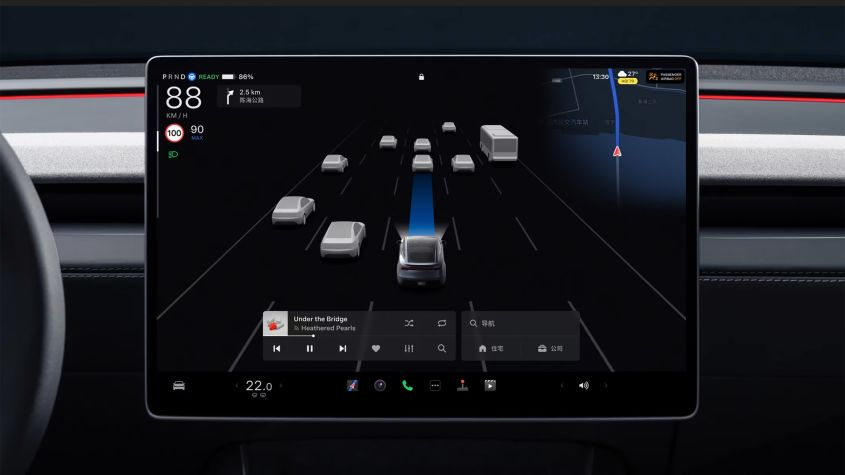
\includegraphics[width=0.45\textwidth]{selfdriving.jpg} &
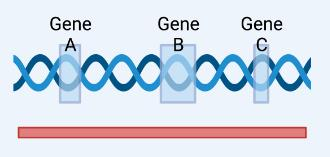
\includegraphics[width=0.45\textwidth]{gene.jpg} \\
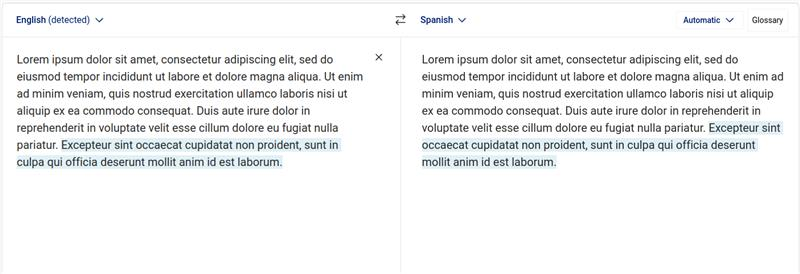
\includegraphics[width=0.45\textwidth]{translation.jpg} &
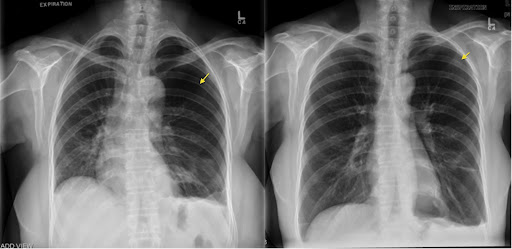
\includegraphics[width=0.45\textwidth]{xray.jpg}
\end{tabular}
\end{center}

\end{frame}

% TODO: some notes on above
Differentiable Programming and Deep Learning give us the ability to computationally solve problems without needing to handcraft the solution or engineer the features. As long as we have data we can build and train models to make predictions.


\begin{frame}
\frametitle{Machine Learning - A Recap}
\mode<presentation>{{\tiny All credit for this slide goes to Niranjan}\par}
\vspace{5mm}
\begin{tabular}{ll}
Data & $\{\bm{x}_n, \bm{y}_n\}^N_{n=1} \qquad \{\bm{x}_n\}^N_{n=1}$
\vspace{3mm} \\ \pause
Function Approximator & $\bm{y} = f (\bm{x}, \bm{\theta})$ %  + \nu
\vspace{3mm} \\ \pause
Parameter Estimation & $E_0 = \sum^N_{n=1} \{\|\bm{y}_n - f (\bm{x}_n; \bm{\theta})\|\}^2$
\vspace{3mm} \\ \pause
Prediction & $\bm{\hat y}_{N+1} = f(\bm{x}_{N+1}, \bm{\hat \theta})$
% \vspace{3mm} \\ \pause
% Regularisation & $E_1 = \sum^N_{n=1} \{\|\bm{y}_n - f (\bm{x}_n; \bm{\theta})\|\}^2 + r(\|\bm\theta\|)$
% \vspace{3mm} \\ \pause
% Modelling Uncertainty & $p(\bm\theta|\{\bm x_n, \bm y_n\}_{n=1}^N)$
% \vspace{3mm} \\ \pause
% Probabilistic Inference & $\mathop{\mathbb{E}}[g(\bm\theta)] = \int g(\bm\theta)p(\bm\theta)d\bm\theta = \frac{1}{N_s}\sum_{n=1}^{N_s}g(\bm\theta^{(n)})$
% \vspace{3mm} \\ \pause
% Sequence Modelling & $\bm x_n = f(\bm x_{n-1}, \bm\theta)$
\end{tabular}
\vspace{5mm}
\end{frame}

\begin{frame}
\frametitle{What is Deep Learning?}

Deep learning is primarily characterised by function compositions: \\ \vspace{10mm}
\begin{itemize}
	\item<2-> Feedforward networks: $\bm{y} = f (g(\bm{x}, \bm\theta_g), \bm{\theta_f})$
	\begin{itemize}
		\item Often with relatively simple functions (e.g. $f(\bm x, \bm{\theta}_f) = \sigma(\bm{x}^\top \bm{\theta}_f)$)
	\end{itemize} \vspace{3mm}
	\item<3-> Recurrent networks: $\bm y_t = f(\bm y_{t-1}, \bm x_t, \bm\theta) = f(f(\bm y_{t-2}, \bm x_{t-1}, \bm\theta), \bm x_t, \bm\theta) = \dots$
\end{itemize}
\vspace{10mm}

\end{frame}

In the early days the focus of deep learning was on learning functions for classification. Nowadays the functions are much more general in their inputs and outputs.


\begin{frame}
\frametitle{What is Differentiable Programming?}

\begin{itemize}
	\mode<article>{\item Differentiable programming is a term coined by Yann Lecun to describe a superset of Deep Learning.}
	\mode<presentation>{
	\item<+-> Captures the idea that computer programs can be partially learned rather than fully programmed by humans.
	\item<+-> The program is made of functions with optimisable parameters.
	}
	\mode<article>{\item<+-> Captures the idea that computer programs can be constructed of parameterised functional blocks in which the parameters are learned using some form of gradient-based optimisation.}
	% \begin{itemize}
		\item<+-> So we need to be able to compute gradients with respect to the parameters of these functional blocks.
		% \item<+-> The idea of Differentiable Programming also opens up interesting possibilities:
		% \begin{itemize}
			\item<+-> The functional blocks don't need to be direct functions in a mathematical sense; more generally they can be \emph{algorithms}.
			\item<+-> What if the functional block we're learning parameters for is itself an algorithm that optimises the parameters of an internal algorithm using a gradient based optimiser?!\footnote{See our ICLR 2019 paper: https://arxiv.org/abs/1812.03928 and NeurIPS 2019 paper: https://arxiv.org/abs/1906.06565}
		% \end{itemize}
	% \end{itemize}
\end{itemize}
\end{frame}

\begin{frame}<article>
\frametitle{Is all Deep Learning Differentiable Programming?}
\begin{itemize}
	\item Not necessarily!
	\begin{itemize}
		\item<+-> Most deep learning systems are trained using first order gradient-based optimisers, but there is an active body of research on gradient-free methods.
		\item<+-> There is an increasing interest in methods that use different styles of learning, such as Hebbian learning, within deep networks. More broadly there are a number of us\footnote{including at least myself, my PhD students and Geoff Hinton!} who are interested in biologically motivated models and learning methods.
		\begin{itemize}
			\item<+-> There's a lot of recent research that computes biological proxies for gradients though!
		\end{itemize}

		\item<+-> This course will primarily focus on differentiable methods, but we'll look at how relaxations can be made to make non-differentiable operators learnable with gradient-based optimisers.
	\end{itemize}
\end{itemize}
\end{frame}

\begin{frame}
	%\frametitle{Where did it all start \& what was the motivation?}
	\frametitle{Success stories - Object detection and segmentation}
	\centering 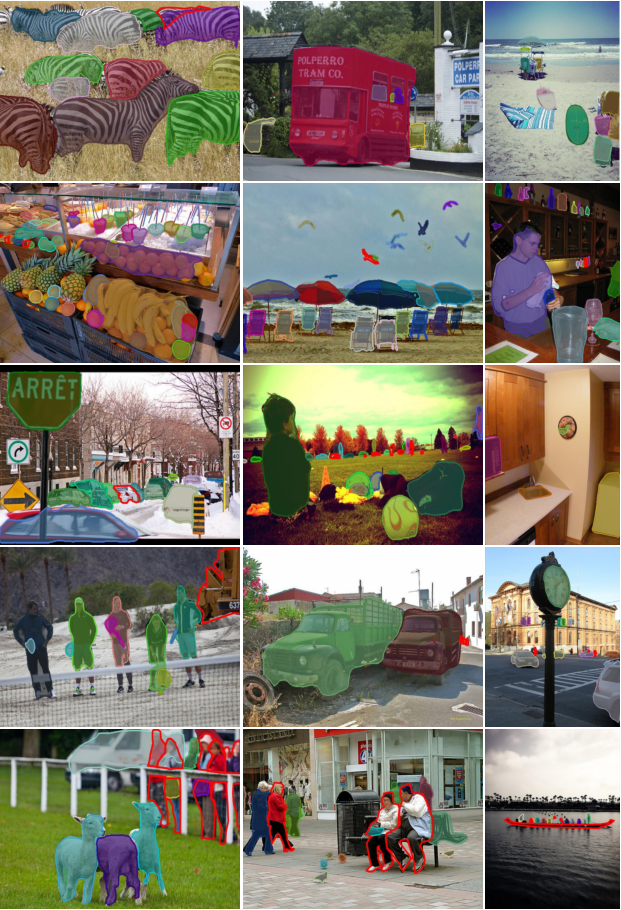
\includegraphics[width=0.3\textwidth]{objseg.pdf}
	\par\footnotesize{Pinheiro, Pedro O., et al. "Learning to refine object segments." European Conference on Computer Vision. Springer, 2016.}
\end{frame}

\begin{frame}
	\frametitle{Success stories - Image generation}
	\centering 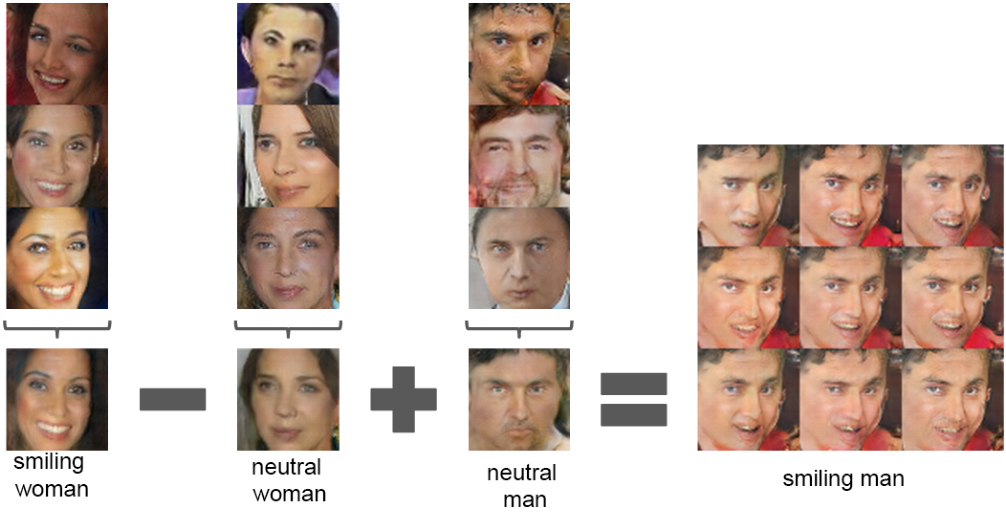
\includegraphics[width=0.8\textwidth]{imggen.pdf}
	\par\footnotesize{Radford, Alec, Luke Metz, and Soumith Chintala. "Unsupervised representation learning with deep convolutional generative adversarial networks." arXiv preprint arXiv:1511.06434 (2015).}
\end{frame}

\begin{frame}
	%\frametitle{Where did it all start \& what was the motivation?}
	\frametitle{Success stories - Translation}

% ENGLISH TEXT\\
% The reason Boeing are doing this is to cram more seats in to make their plane
% more competitive with our products," said Kevin Keniston, head of passenger
% comfort at Europe's Airbus.
% \\[1em]
% TRANSLATED TO FRENCH\\
% La raison pour laquelle Boeing fait cela est de creer plus de sieges pour rendre
% son avion plus competitif avec nos produits", a declare Kevin Keniston, chef
% du confort des passagers chez Airbus. \blfootnote{Wu, Yonghui, et al. "Google's neural machine translation system: Bridging the gap between human and machine translation." arXiv preprint arXiv:1609.08144 (2016).}

\centering 
\includegraphics[]{translation.pdf}
\par\footnotesize{Lyu, C., Du, Z., Xu, J., Duan, Y., Wu, M., Lynn, T., Aji, A.F., Wong, D.F., Liu, S. and Wang, L., 2023. A Paradigm Shift: The Future of Machine Translation Lies with Large Language Models. LREC-COLING 2024}
\end{frame}

Language translation has made massive leaps over the last 10 years as a result of deep learning. Initially this was because of large aligned datasets and translation models that targeted transforming a sequence of words in one language to another. As a result of large language models we are increasingly seeing translation quality improve in terms of the nuance and subjective feel of the translation --- translations are starting to becoming more natural and less mechanistic (but possibly less objectively accurate as a result).

\begin{frame}
	\frametitle{Why should we care about this?}
		\centering
		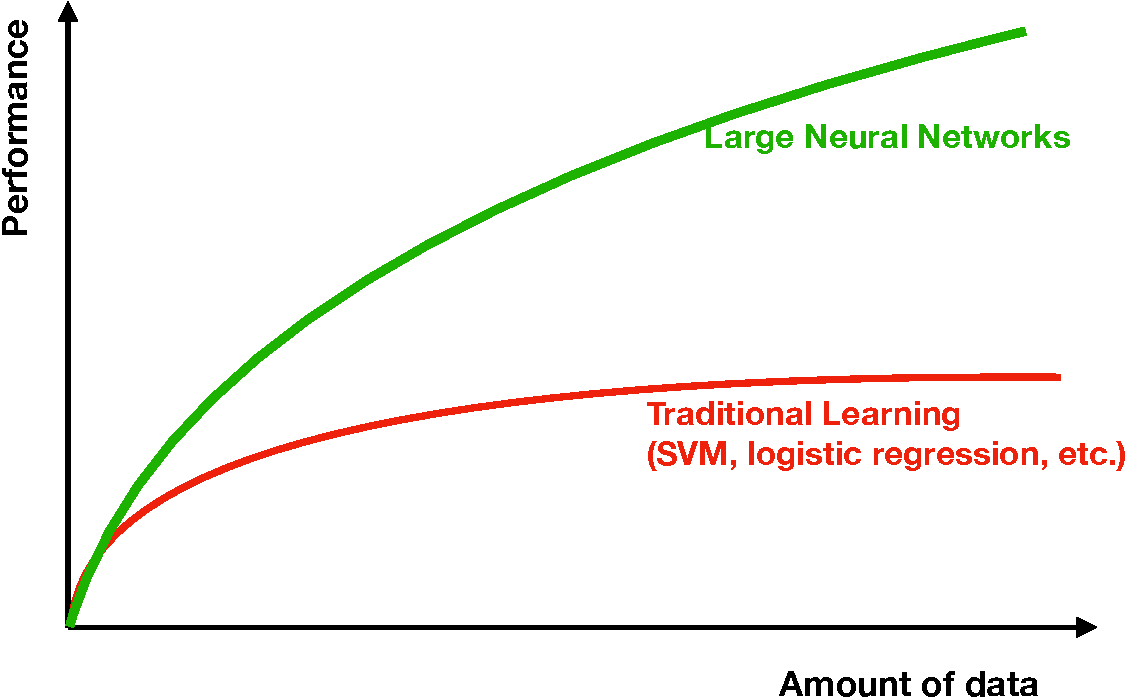
\includegraphics[width=0.9\textwidth]{Fig1.pdf}
		\par\footnotesize{Image courtesy of Andrew Ng}
\end{frame}

The above picture shows how model performance has been shown to be linked to the amount of data. The story of the last 10-15 years has been one of increasingly growing data. Traditional approaches to machine learning have largely not scaled in performance in the same way large deep neural networks have. This is predominantly because of the way features are extracted from the data; traditional machine learning often used hand-crafted features, whereas the story of deep learning is all about feature learning --- giving the model essentially raw data and letting it learn to appropriate features to make decisions from. 

We should recognise however that traditional methods still have their place - when datasets are small, and perhaps there isn't much feature engineering to do, they can and do outperform deeper models. At the same time, a large proportion of deep network architectures are themselves nothing more than a learned linear model (linear regression, logistic regression, SVM, ...) attached to a learned feature extractor, so those very basic traditional methods are still very much a big part of the picture today!

\begin{frame}
	\frametitle{Key takeaways}

	\begin{itemize}
		\item<+-> \textbf{More data availability} in all domains...
		\item<+-> ...allows for \textbf{bigger/deeper/more complex models}
		\item<+-> ...models that can \textbf{learn the features}
		\item<+-> and these can have far \textbf{greater performance}
	\end{itemize}
\end{frame}

\begin{frame}
	\frametitle{What is the objective of this module?}

	\textbf{A word of warning: This is not a module about how to apply someone else's deep network architecture to a task, or how to train existing models!}
	\\[1em]
	You will learn some of that along the way of course, but the real objective is for you to graduate knowing how to understand, critique and implement new and recent research papers on deep learning and associated topics.
\end{frame}

\begin{frame}
	\frametitle{What is the objective of this module?}
	\begin{itemize}
		\item<+-> Understand the underlying mathematical and algorithmic principles of deep learning.
		\item<+-> Apply deep learning methods to real datasets.
		\item<+-> Learn how to train models using deep learning libraries.
		\item<+-> Think critically about upcoming research in deep learning.
		
		% \item<+-> Understand the key factors that have made differentiable programming successful for various applications.
		% \item<+-> Apply existing deep learning models to real datasets.
		% \item<+-> Gain facility in working with deep learning libraries in order to create and evaluate network architectures.
		% \item<+-> Critically appraise the merits and shortcomings of model architectures on specific problems.
		% \item<+-> Have a technical and mathematical grounding that enables you to understand the field as it rapidly evolves.
		% \item<+-> Find out about some of the research going on here!
	\end{itemize}
\end{frame}

\begin{frame}
	\frametitle{How is this module going to be delivered?}

	\begin{itemize}
		\item<+-> Lectures (3 per week except when we have seminars)
		\begin{itemize}
			\item Note: We are refreshing some material from last year, but the website may have old links.
			\item You need to read the suggested papers/links before the lectures!
			\item There is maybe a little room for some flexibility later in the course on topics - tell us what you're interested in!
			\item<+-> Lectures will be face to face, but also recorded for the website when possible (do not rely on this!).
		\end{itemize}
	\end{itemize}
\end{frame}

\begin{frame}
	\frametitle{How is this module going to be delivered?}

	\begin{itemize}
		\item<+-> Seminars (4)
		\begin{itemize}
			\item We'll look at a particular paper, papers or ideas in some detail and have an open discussion
			\item You'll need to prepare in advance \& be ready to ask questions and share your thoughts
			\item Not recorded, but contents examinable in the quizzes
		\end{itemize}
	\end{itemize}
\end{frame}

\begin{frame}
	\frametitle{How is this module going to be delivered?}

	\begin{itemize}
		\item<+-> Labs (1x 2 hour session per week for 8 weeks + additional help sessions if required)
		\begin{itemize}
			\item Labs consist of a number of Juypter notebooks you will work though.
			\begin{itemize}
				\item You'll be using PyTorch as the primary framework, with Torchbearer to help out.
				\item You will need to utilise GPU-compute for the later labs (we provide Google Colab links so you can use NVidia K80s or newer in the cloud).
			\end{itemize}
			\item Labs are in-person (Zepler L3) with a team of PhD student demonstrators \& myself and/or Antonia.
			\item Please ask lots of questions and use this time to get help on the labs and coursework.
			\item After each lab you will have to do a follow-up problem-sheet exercise that will be marked.
		\end{itemize}
	\end{itemize}
\end{frame}

\begin{frame}
	\frametitle{What will we cover in the module?}
	\url{https://ecs-vlc.github.io/COMP6258/}
\end{frame}

\begin{frame}
	\frametitle{Lab session plan}

	\begin{center}
	\begin{tabular}{ l l l }
		 Lab & Date & Topic \\ \hline
		 Lab 1  & 31/01/25 & Introducing PyTorch \\
		 Lab 2  & 07/02/25 & Automatic Differentiation \\
		 Lab 3  & 14/02/25 & Optimisation \\
		 Lab 4  & 21/02/25 & NNs with PyTorch and Torchbearer \\
 		 Lab 5  & 28/02/25 & CNNs with PyTorch and Torchbearer \\
 		 Lab 6  & 07/03/25 & Transfer Learning \\
 		 Lab 7  & 14/03/25 & RNNs, Sequence Prediction and Embeddings \\
     Lab 8  & 21/03/25 & Deep Generative Models\\
     Lab 9  & 28/03/25 & (catch-up/questions)\\
	\end{tabular}
	\end{center}
\end{frame}

\begin{frame}
	\frametitle{What do we expect you already know?}

	\begin{itemize}
	\item<+-> COMP3223 or COMP6245 (fundamentals of statistical learning, MLPs, gradient descent, how to train and evaluate learning machines, supervised-vs-unsupervised)
	\item<+-> Fundamentals of:
	\begin{itemize}
		\item Matrix Algebra (matrix-matrix, matrix-vector and matrix-scalar operations, inverse, determinant, rank, Eigendecomposition, SVD);
		\item Probability \& Statistics (1st-order summary statistics, simple continuous and discrete probability distributions, expected values, etc); and,
		\item Multivariable Calculus (partial differentiation, chain-rule).
	\end{itemize}
	\item<+-> Programming in Python
	\end{itemize}
\end{frame}

\begin{frame}
	\frametitle{What might you already know?}
	\begin{itemize}
	\item<+-> How to use a deep learning framework (Keras, Tensorflow, PyTorch)?
	\item<+-> How to train an existing model architecture using a GPU?
	\item<+-> How to perform transfer learning?
	\item<+-> How to perform differentiable sampling of a Multivariate Normal Distribution?
	\end{itemize}
\end{frame}

\begin{frame}
	\frametitle{Assessment Structure}
	\begin{itemize}
		\item Interim project plan - Handin in week 5 (26th Feb, 4PM)
		\item Lab work $40\%$ - Handin in week 11 (7th May, 4PM)
		\item Online quizzes $20\%$ - Planned for week 6 (5th March) and week 12 (14th May)
		\item Final project $40\%$  - Handin in week 12 (16th May, 4PM)
	\end{itemize}
\end{frame}

\begin{frame}
	\frametitle{The Main Assignment}
	\framesubtitle{The COMP6258 Reproducibility Challenge}
	\url{https://ecs-vlc.github.io/COMP6258/coursework.html}
\end{frame}

\end{document}
